\chapter{Chromatin Accessibility During Development in \emph{Drosophila pseudoobscura}}

\hrulefill

\section{Experimental Motivation and Design}

Despite having distinct DNA binding domains and preferences for specific sequence motifs, many developmental transcription factors show surprisingly similar genome-wide binding patterns in \emph{D. melanogaster} embryos, differing primarily in quantitative levels of occupancy at a highly-overlapping set of genomic regions \citep{macarthur_developmental_2009}. Both experimental evidence and computational modelling have revealed an important role for chromatin accessibility in determining these overlapping bound regions \citep{kaplan_quantitative_2011, li_role_2011}. Patterns of chromatin accessibility in embryonic nuclei change throughout development as cells take on more committed fates, allowing transcription factors access to different regions of regulatory DNA and ultimately contributing to overall body patterning \citep{thomas_dynamic_2011}. The importance of chromatin accessibility in directing patterns of transcription factor binding has also been observed in \emph{Drosophila} imaginal discs as well as in mammalian cells \citep{john_chromatin_2011, mckay_common_2013, neph_expansive_2012}. Since a major goal of this thesis was to examine differences in transcription factor binding between \emph{Drosophila} species, I was interested in measuring chromatin accessibility during development of non-model drosophilids in order to determine whether observed differences in TF binding could be correlated with differences in accessibility.\\
   
Two major techniques exist to detect genome-wide patterns of chromatin accessibility \emph{in vivo}: DNase-seq and FAIRE-seq. DNase-seq relies on the non-specific digestion of chromatin by the enzyme DNaseI. Nuclei are isolated and immediately treated with DNaseI, which cleaves DNA wherever it is accessible. Short DNA fragments resulting from these cleavages are then recovered and sequenced, leading to the identification of DNase-hypersenstive sites (DHS) \citep{thomas_dynamic_2011}. Although this technique has been used extensively, there is some evidence that DHS datasets may suffer from bias due to sequence preferences of DNaseI, which may vary depending on the experimental conditions \citep{koohy_chromatin_2013}. An alternative technique is FAIRE-seq (Formaldehyde-Assisted Identification of Regulatory Elements). In FAIRE-seq, nuclei are isolated and fixed with formaldehyde. The chromatin is then sonicated, breaking the more accessible regions into small fragments, and purified using phenol-chloroform extractions. This results in only DNA from accessible regions being recovered, as inaccessible, compacted chromatin is left in the organic phase during the extractions \citep{giresi_isolation_2009, simon_using_2012}. Although DNase-seq and FAIRE-seq do not perfectly recapitulate each other, as DNAse-seq tends to detect a higher signal at promoter regions while FAIRE-seq tends to detect a higher signal at distal regulatory regions, overall the two techniques show good correspondence \citep{koohy_chromatin_2013, mckay_common_2013}.\\
   
I decided to use FAIRE-seq to study chromatin accessibility and to focus on one species, \emph{D. pseudoobscura}, which is the most distant species to \emph{D. melanogaster} of those that I studied and which shows the greatest difference in chromosomal structure and arrangement \citep{clark_evolution_2007,richards_comparative_2005}. I performed FAIRE-seq on \emph{D. pseudoobscura} embryonic chromatin from five developmental stages, stage 5, stage 9, stage 10, stage 11 and stage 14, chosen to provide a comparison with \emph{D. melanogaster} DNase-seq data from Thomas et al. (2011). The timing of each developmental stage in \emph{D. pseudoobscura} was calculated according to \citet{kuntz_native_2013}; more details are available in Chapter 2. I sequenced three biological replicates from each stage. Although input chromatin can be used as a control for FAIRE-seq, as with ChIP-seq, it is not strictly necessary \citep{simon_using_2012}. Indeed, as one of the sources of the non-random patterns of reads observed in input controls is chromatin accessibility, it is possible that using such a control with FAIRE-seq would reduce the detection of true FAIRE signal. For my FAIRE-seq experiments, I did not sequence matched input controls for each developmental stage, but rather used GC-content and mappability data calculated from the \emph{D. pseudoobscura} genome to correct for potential biases in the data during analysis. A detailed description of the methods used in the FAIRE protocol and for processing the sequencing data can be found in Chapter 2.

\section{Overview of FAIRE-seq results}
A summary of the clean and uniquely mapped reads as well as the rate of duplicate reads for each sample can be found in Table 6.1. The rates of duplication for these datasets range from 10.5 - 16.6\%; however, the majority of the duplicates are only 2-fold, indicating high-quality, high-complexity libraries overall. Visualization of the read density scores across the genome shows a mix of regions with very strong, high peaks and regions with a much lower signal-to-noise ratio. High reproducibility is observed between biological replicates from the same stage, as well as a high degree of similarity between stages (Figure 6.1).\\

\begin{figure}
\centering
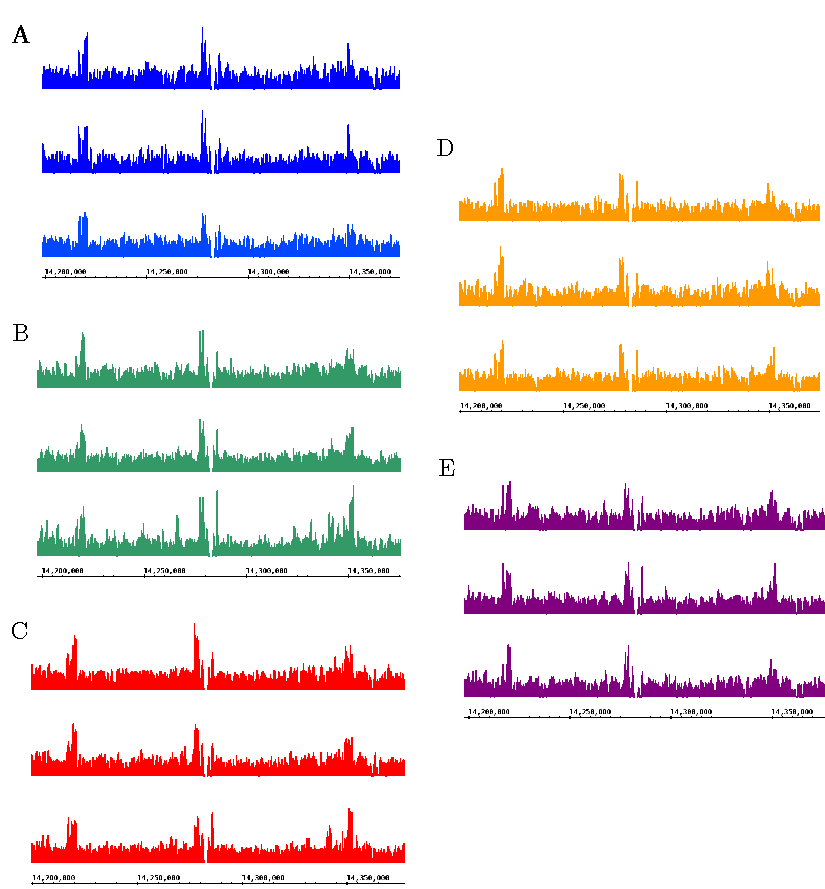
\includegraphics{fig6-1}
\caption{Comparison of read profiles between FAIRE biological replicates and developmental stages. The same 175-kb region of chromosome 2 in \emph{D. pseudoobscura} is shown for each stage. In all samples, a relatively small number of strong, highly reproducible peaks are present, as well as smaller, less reproducible peaks which may constitute background noise. In all cases, reads have been normalized to a total library size of 1,000,000 for visualization purposes. The y-axes range from 0-15 reads. A.) Stage 5, three biological replicates. B.) Stage 9, three biological replicates. C.) Stage 10, three biological replicates. D.) Stage 11, three biological replicates. E.) Stage 14, three biological replicates.}
\label{Figure 6.1}
\end{figure}

\begin{table}[h]
\centering
\begin{tabular}{|l|l|l|l|}
\hline
\textbf{Sample}      & \textbf{Clean reads} & \textbf{Mapped reads} & \textbf{\% Duplicate reads} \\ \hline
Stage 5\_1  & 14,316,011    & 7,693,543      & 12.72              \\ \hline
Stage 5\_2  & 7,160,440     & 5,073,937      & 10.52              \\ \hline
Stage 5\_3  & 11,116,549    & 9,115,838      & 12.67              \\ \hline
Stage 9\_1  & 10,665,720    & 8,708,489      & 12.73              \\ \hline
Stage 9\_2  & 10,451,702    & 8,782,095      & 12.00               \\ \hline
Stage 9\_3  & 10,476,067    & 8,891,655      & 12.79              \\ \hline
Stage 10\_1 & 12,937,965    & 7,749,216      & 13.03              \\ \hline
Stage 10\_2 & 11,122,744    & 9,629,801      & 12.47              \\ \hline
Stage 10\_3 & 10,356,274    & 8,987,571      & 12.36              \\ \hline
Stage 11\_1 & 11,459,640    & 9,950,997      & 13.81              \\ \hline
Stage 11\_2 & 11,148,754    & 9,635,232      & 13.35              \\ \hline
Stage 11\_3 & 8,897,559     & 7,727,392      & 12.64              \\ \hline
Stage 14\_1 & 10,336,055    & 8,988,933      & 13.42              \\ \hline
Stage 14\_2 & 9,947,079     & 8,639,987      & 12.94              \\ \hline
Stage 14\_3 & 14,637,840    & 12,291,220     & 15.65              \\  \hline
\end{tabular}
\caption{Summary of reads produced for FAIRE-seq libraries}
\label{Table 6.1}
\end{table}

After mapping and extending reads, peaks were called for each replicate separately using MOSAiCS \citep{chung_mosaics_2012}. Peaks from each replicate were combined to make a high-confidence set for each stage by keeping all peaks that are present in 2 out of 3 replicates at FDR10. After merging peaks that were overlapping or immediately adjacent, this resulted in a set of 6348 total unique peaks across all stages. The number of peaks called at FDR5 and FDR10 for each replicate, as well as the combined peaks and unique peaks for each developmental stage are shown in Table 6.2. A large number of peaks for each stage are mapped to unassembled regions (chrU); while these peaks are likely to represent legitimate regions of accessible chromatin, they could map to repetitive regions and are, unfortunately, more difficult to annotate than peaks in assembled chromosomes.\\

\begin{table}[h]
\centering
\begin{tabular}{|l|l|l|p{2cm}|p{2cm}|}
\hline
\textbf{Sample}            & \textbf{FDR5 peaks} & \textbf{FDR10 peaks} & \textbf{Combined peaks} & \textbf{Unique peaks} \\ \hline
Stage 5\_1        & 4600       & 5208        &                &              \\ \hline
Stage 5\_2        & 4209       & 4685        &                &              \\ \hline
Stage 5\_3        & 4527       & 5100        &                &              \\ \hline
\textbf{Stage 5 combined}  &            &             & \textbf{4607}           & \textbf{212}          \\ \hline
Stage 9\_1        & 4714       & 5326        &                &              \\ \hline
Stage 9\_2        & 4087       & 4490        &                &              \\ \hline
Stage 9\_3        & 7010       & 7979        &                &              \\ \hline
\textbf{Stage 9 combined}  &            &             & \textbf{5165}           & \textbf{475}          \\ \hline
Stage 10\_1       & 6102       & 6966        &                &              \\ \hline
Stage 10\_2       & 4175       & 4599        &                &              \\ \hline
Stage 10\_3       & 4697       & 5238        &                &              \\ \hline
\textbf{Stage 10 combined} &            &             & \textbf{5102}           & \textbf{316}          \\ \hline
Stage 11\_1       & 4520       & 5059        &                &              \\ \hline
Stage 11\_2       & 4008       & 4423        &                &              \\ \hline
Stage 11\_3       & 4378       & 4837        &                &              \\ \hline
\textbf{Stage 11 combined} &            &             & \textbf{4444}           & \textbf{185}          \\ \hline
Stage 14\_1       & 4514       & 4988        &                &              \\ \hline
Stage 14\_2       & 4355       & 4794        &                &              \\ \hline
Stage 14\_3       & 4287       & 4739        &                &              \\ \hline
\textbf{Stage 14 combined} &            &             & \textbf{4674}           & \textbf{288}          \\ \hline
\end{tabular}
\caption{Peaks called in each FAIRE-seq replicate as well as combined and unique peaks for each developmental stage.}
\label{Table 6.2}
\end{table}

\begin{figure}
\centering
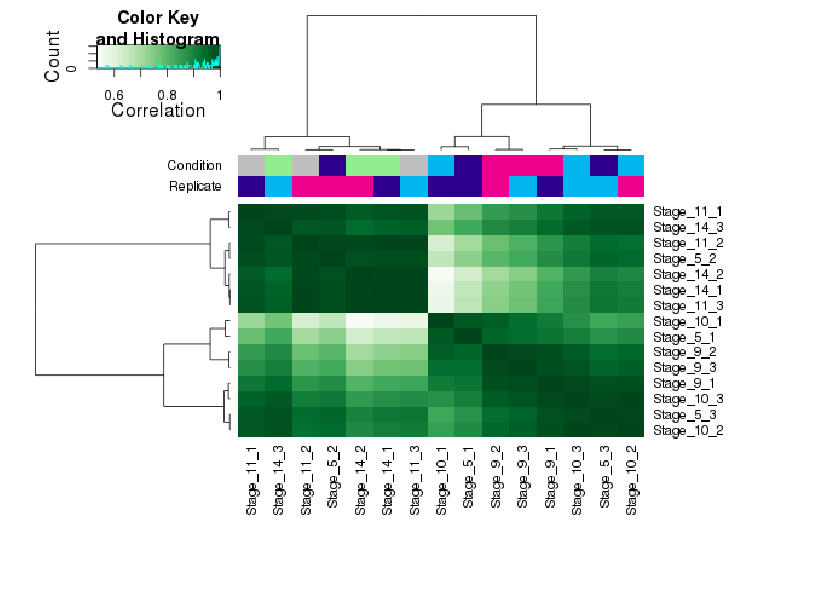
\includegraphics{fig6-2}
\caption{Heatmap showing clustering of all FAIRE-seq samples by affinity scores in every FAIRE interval. None of the stages has all three biological replicates clustered together. However, a division is visible between earlier stages (5, 9 and 10, in lower right) and later stages (11 and 14, in upper left), with the exception of stage 5 replicate 2, which clusters with the later stages. The color key and histogram show the distribution of pairwise correlations between sample affinity scores. Darker green corresponds to a higher correlation, while lighter green corresponds to a lower correlation.}
\label{Figure 6.2}
\end{figure}

In general the read density profiles for replicate stages are highly correlated; however, there is some between-replicate variability. In particular, replicate 2 for stage 5 is an outlier compared to the other stage 5 replicates. Clustering of each replicate by read counts within peaks shows that the two later stages are highly similar and can be differentiated from the earlier stages, with the stage 11 and stage 14 replicates clustering together and the stage 5, stage 9 and stage 10 replicates (except for Stage 5\_2) clustering together (Figure 6.2). A similar effect can be seen in a principal component analysis (PCA) plot (Figure 6.3); the stage 11 and stage 14 replicates form a cluster together which is separable from the stage 9 samples, while the stage 5 and stage 10 replicates, which show greater within-stage variability, are spread across both principal component axes. Using DiffBind to identify differentially enriched sites between each stage and then clustering the replicates based only on those differential sites reveals a tighter clustering within the stage 11 samples and the stage 9 samples but greater variability within the stage 5, stage 10 and stage 14 samples (Figure 6.4) \citep{ross-innes_differential_2012}.\\

\begin{figure}
\centering
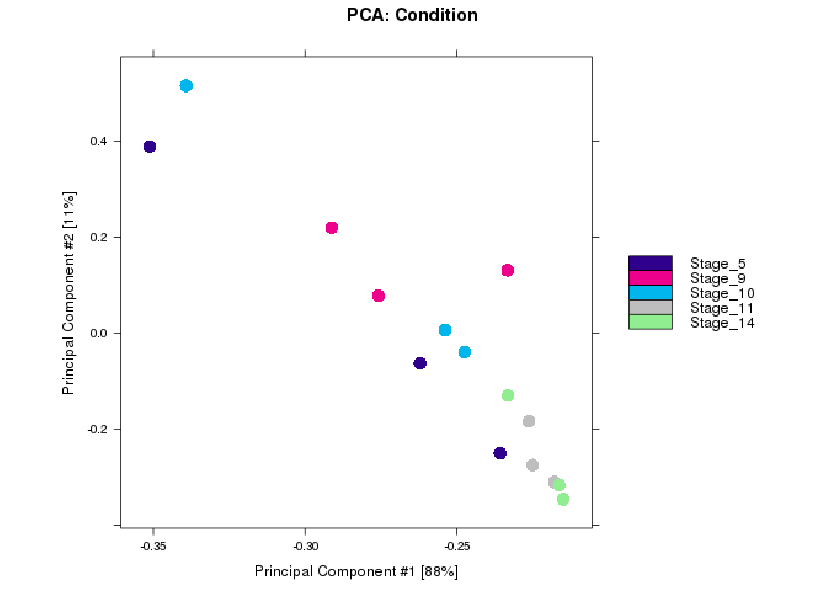
\includegraphics[width=9cm]{fig6-3}
\caption{Principal component analysis of all FAIRE-seq samples. The first principal component, which explains 88\% of the variation among samples, is plotted on the x-axis, and the second principal component, which explains 11\% of the variation among samples, is plotted on the y-axis. As with the heatmap, a division is visible between earlier stages (5, 9 and 10) and later stages (11 and 14), although the replicates from later stages cluster more tightly than the replicates from earlier stages.}
\label{Figure 6.3}
\end{figure}

\begin{figure}
\centering
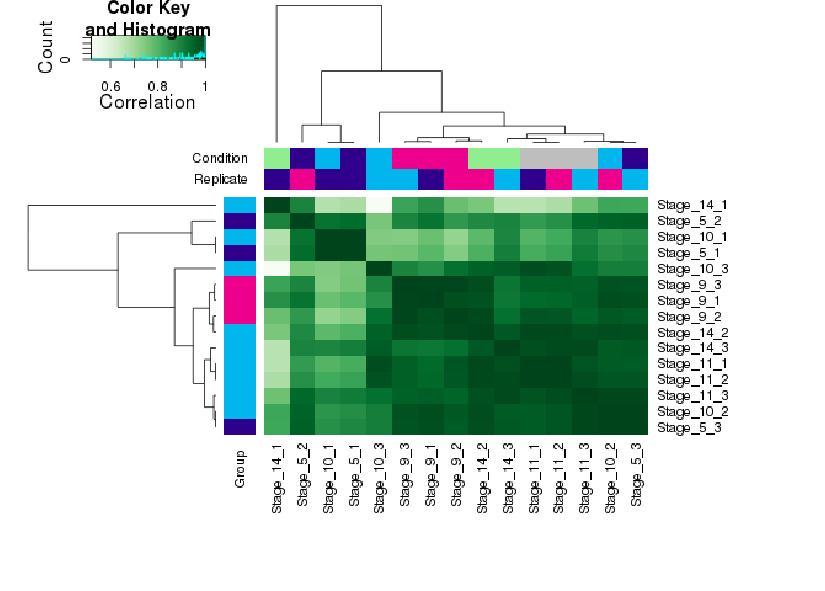
\includegraphics{fig6-4}
\caption{Heatmap showing clustering of all FAIRE-seq samples by affinity scores in FAIRE intervals that are differentially enriched in each stage in relation to the others. The three biological replicates from stage 9 cluster together along with one stage 14 replicate, while the other stages show greater variability between replicates. The color key and histogram show the distribution of pairwise correlations between sample affinity scores. Darker green corresponds to a higher correlation, while lighter green corresponds to a lower correlation.}
\label{Figure 6.4}
\end{figure}

Individual sites show a high level of persistence between developmental stages, although some sites are gained and lost at each stage (Figure 6.5). Stage 9 has the highest percentage of sites that are not present in the previous stage and therefore originate in that stage (21.5\%). Of the high-confidence accessible sites present at stage 14, 84\% are present in stage 5, with 5.1\% originating in stage 9, 1.8\% originating in stage 10, 2.5\% originating in stage 11, and 6.2\% originating uniquely in stage 14. In accordance with this high persistence of accessible sites throughout development, DiffBind found relatively low numbers of sites with differential enrichment of read counts between stages, in particular when comparing between early stages (5, 9, and 10) or between late stages (11 and 14) (Table 6.3). It should be noted, however, that because these differentially enriched sites are based on read counts that are normalized between samples, while peaks were initially called based on the read density profiles from each sample independently, the numbers of unique peaks and the numbers of differentially enriched peaks for each stage are not directly comparable.\\

\begin{figure}
\centering
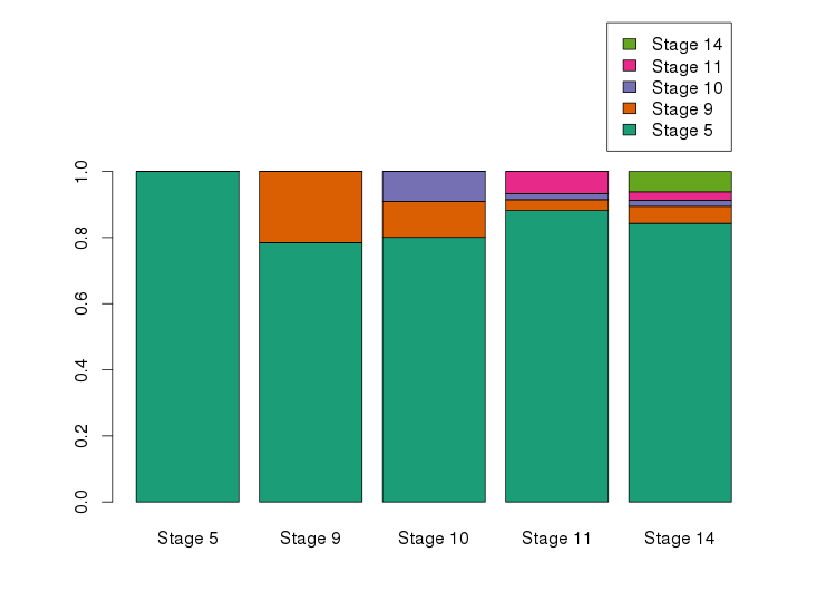
\includegraphics[width=10cm]{fig6-5}
\caption{FAIRE intervals in each stage by stage of origin. For all intervals in each developmental stage, the earliest stage in which the interval is present was determined. The majority of FAIRE sites are present starting in stage 5 through stage 14, and a smaller proportion originate in each stage. The proportion of sites originating in each stage after stage 5 decreases over the course of development.}
\label{Figure 6.5}
\end{figure} 

\begin{table}[h]
\centering
\begin{tabular}{|l|l|l|}
\hline
\textbf{1st stage} & \textbf{2nd stage} & \textbf{Differential peaks} \\ \hline
Stage 5   & Stage 9   & 4                  \\ \hline
Stage 5   & Stage 10  & 0                  \\ \hline
Stage 5   & Stage 11  & 23                 \\ \hline
Stage 5   & Stage 14  & 111                \\ \hline
Stage 9   & Stage 10  & 2                  \\ \hline
Stage 9   & Stage 11  & 1581               \\ \hline
Stage 9   & Stage 14  & 1028               \\ \hline
Stage 10  & Stage 11  & 608                \\ \hline
Stage 10  & Stage 14  & 488                \\ \hline
Stage 11  & Stage 14  & 5                  \\ \hline
\end{tabular}
\caption{Peaks with differential enrichment in pairwise comparisons between developmental stages.}
\label{Table 6.3}
\end{table}

\section{Functional analysis of FAIRE peaks}
\subsection{Genomic annotation of FAIRE peaks}
One of the challenges of working with non-model species is the relative lack of genome annotations available. In order to examine the genomic distribution of FAIRE peaks, I downloaded gene predictions made by both Genscan and GeneID from the UCSC Table Browser \citep{burge_prediction_1997,karolchik_ucsc_2004, karolchik_ucsc_2014,parra_geneid_2000}. I used these to annotate each FAIRE peak to either an exon, exon border, intron, gene border (5’ or 3’), or intergenic region. The percentages of peaks annotated to each type of genomic region are very similar between all stages using each set of gene predictions. Of the total unique peaks, using the Genscan predictions, 3.7\% fall entirely within exons, 30\% fall on exon borders, 14.6\% fall entirely within introns, 15.5\% fall on gene borders and 36.1\% fall entirely within intergenic regions (Figure 6.6A). Using the GeneID predictions, 2.8\% fall entirely within exons, 20\% fall on exon borders, 28.8\% fall entirely within introns, 11.8\% fall on gene borders and 36.5\% fall entirely within intergenic regions (Figure 6.6B). The main difference between annotations made with the Genscan and GeneID predictions is between the exon border, intron, and gene border categories, suggesting that while the exact locations of gene and exon predictions vary between the two predicted gene sets, the overall proportion of FAIRE peaks hitting genes and exons is similar.

\begin{figure}
\centering
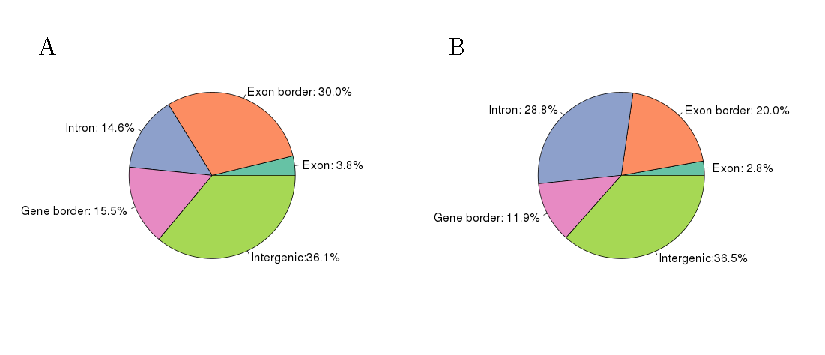
\includegraphics{fig6-6}
\caption{Genomic annotation of FAIRE sites. For each set of annotations, five genomic feature categories were considered: intron, exon, exon border, gene border and intergenic. All unique FAIRE sites, from all stages, were annotated. A.) Annotations based on Genscan gene models. The majority of FAIRE sites fall into intergenic regions, followed by exon borders and gene borders. Both the intergenic and gene border categories may include promoters. B.) Annotations based on GeneID gene models. The proportion of FAIRE sites in intergenic regions and exons is similar to that for Genscan annotations, but more sites are annotated to introns and less to gene borders and exon borders.}
\label{Figure 6.6}
\end{figure}

\subsection{Enriched motifs in FAIRE peaks}
To identify enriched sequence motifs within FAIRE peaks in an unbiased way, I used HOMER to perform scans for both \emph{de novo} motifs and known motifs \citep{heinz_simple_2010}. All stages showed similar motif enrichments. For each stage, the top hits of known motifs included a helix-loop-helix (HLH) motif (p \textless 1e-26), a basic leucine zipper (bZIP) motif (p \textless 1e-21) and a zinc-finger domain (zf) motif (p \textless 1e-11), as well as several motifs flagged as promoters, including the TATA-box motif (p \textless 1e-6). 15-16\% of peaks in all stages contained a TATA-box motif, indicating a strong presence of promoter regions in the recovered FAIRE intervals. Although none of the promoter motifs identified in the Thomas et al. DNase-seq data were enriched in my datasets, the FAIRE peaks at each stage were enriched for multiple known promoter sequences according to HOMER \citep{thomas_dynamic_2011}. The TATA motif was also flagged as enriched in \emph{de novo} motif analyses, with one of the top-hit and most highly significant motifs in each stage being a GAGATATA motif (p \textless= 1e-135) (Figure 6.7A). The best match for this motif among curated \emph{Drosophila} motifs found using STAMP is Chorion factor 1 (Cf1), a zinc-finger transcription factor with a functional annotation of RNA polymerase II core promoter proximal region sequence-specific DNA binding activity \citep{mahony_stamp:_2007}. Another highly significant motif found in de novo analysis was difficult to assign to a known \emph{Drosophila} transcription factor; however, its closest match was for Knirps (Kni) (p \textless= 1e-136) . As kni is a member of the nuclear hormone receptor (NHR) family, this motif may reflect general NHR activity in FAIRE intervals (Figure 6.7B).\\

\begin{figure}
\centering
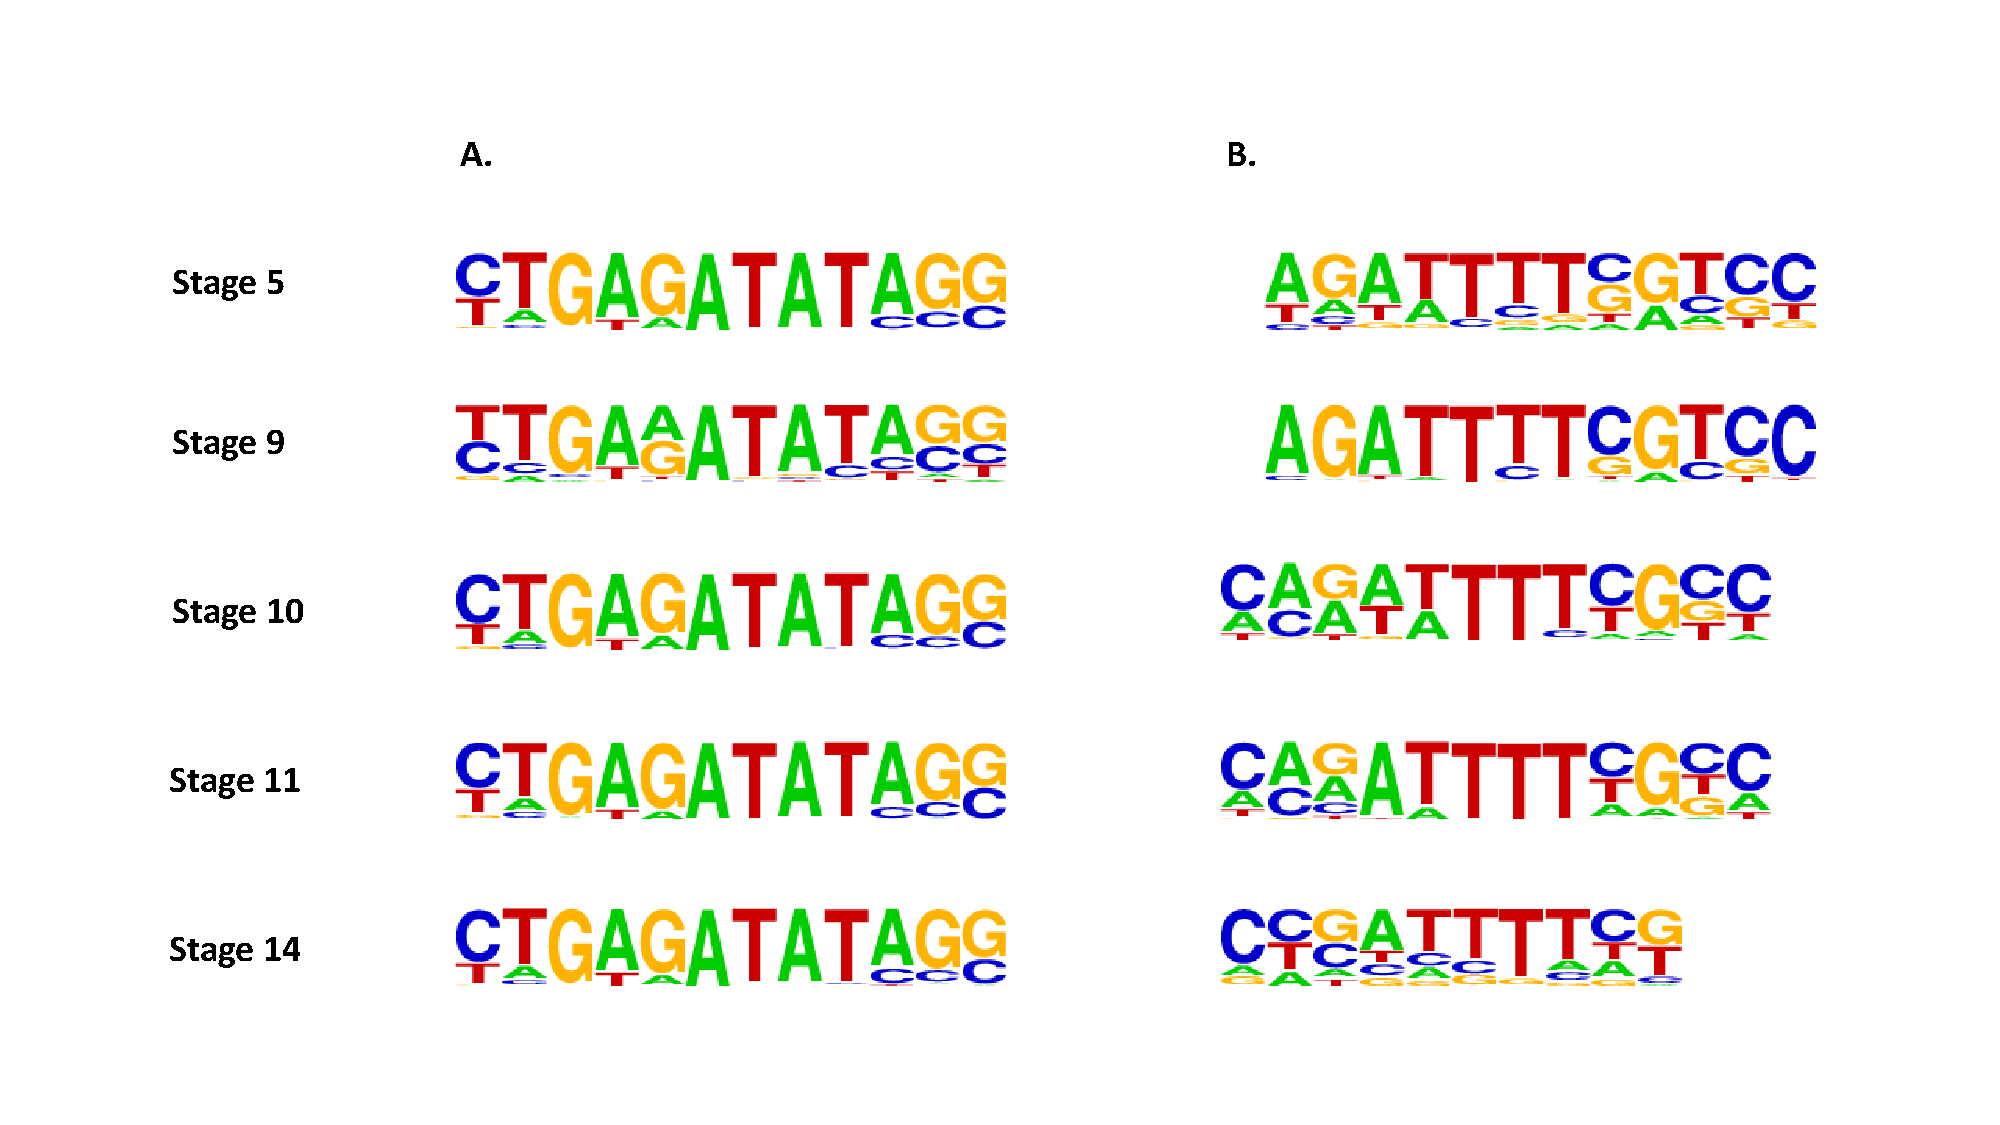
\includegraphics[width=13.97cm]{fig6-7}
\caption{Two of the top \emph{de novo} motifs identified in FAIRE intervals at every stage. A.) A highly significant GAGATATA motif, which may correspond to Cf1 binding in promoter regions, is found in all stages (p <= 1e-135). B.) A motif potentially matching Kni, which may represent nuclear hormone receptor activity, is found in all stages (p <= 1e-136).}
\label{Figure 6.7}
\end{figure}

Many of the top \emph{de novo} motifs are predicted by HOMER to match non-\emph{Drosophila} TFs, including vertebrate, yeast, and plant TFs. However, these motifs are highly significant, and, given the high percentages of reads that mapped to the \emph{D. pseudoobscura} genome, they are unlikely to be the result of contamination by DNA from other species. The predicted TF reported by HOMER for each motif is only a best guess and is dependent on the motifs available in the databases queried, meaning that true matches could be missed. It is possible that these motifs represent promoter elements or other deeply conserved features of open chromatin. A summary of the top ten \emph{de novo} motifs identified in each stage can be found in Table 6.4.\\

\begin{center}
\begin{longtable}{|l|l|l|l|l|}
\hline
\textbf{Stage}    & \textbf{Rank} & \textbf{Predicted TF}  & \textbf{Consensus sequence} & \textbf{P-value} \\ \hline
\endfirsthead

\caption[Top ten de novo motifs by p-value in FAIRE peaks from each stage. For each motif, the TF predicted by HOMER, the consensus sequence and the p-value are shown.]{Top ten de novo motifs by p-value in FAIRE peaks from each stage. For each motif, the TF predicted by HOMER, the consensus sequence and the p-value are shown.} \label{Table 6.4} \\
\endlastfoot

Stage 5  & 1    & Pan           & AGATTTTSGTCC       & 1E-163  \\ \hline
         & 2    & E2F3          & YGYGAKCGGAAR       & 1E-162  \\ \hline
         & 3    & SIG1          & CCTATATCTCAG       & 1E-146  \\ \hline
         & 4    & STP3          & GCTAGAGCAACG       & 1E-136  \\ \hline
         & 5    & Hand1::Tcfe2a & AGTCTGGATC         & 1E-136  \\ \hline
         & 6    & Hbp1\_2       & CGAAAATGGG         & 1E-130  \\ \hline
         & 7    & MATA1         & GCATCCACAATT       & 1E-127  \\ \hline
         & 8    & XBP1          & CTCAAAGACTAT       & 1E-117  \\ \hline
         & 9    & Ovo           & CTTCTGTKAKAT       & 1E-111  \\ \hline
         & 10   & ZmHOX2a       & AGGGCCCGATCG       & 1E-109  \\ \hline
Stage 9  & 1    & ARR10         & AGATTTTCGTCC       & 1E-158  \\ \hline
         & 2    & SIG1          & CCTATATYTCAR       & 1E-142  \\ \hline
         & 3    & Smad3\_1      & RGAKCCAGACTS       & 1E-142  \\ \hline
         & 4    & MET31         & TTCGCCSCACTY       & 1E-132  \\ \hline
         & 5    & Btd           & CTTCCGCCCCCA       & 1E-132  \\ \hline
         & 6    & ZmHOX2a       & CGATCGGGCCCT       & 1E-115  \\ \hline
         & 7    & MATA1         & GCATCCACAATT       & 1E-110  \\ \hline
         & 8    & CST6          & GTRACATC           & 1E-101  \\ \hline
         & 9    & Pros          & KAGTCMTGCC         & 1E-099  \\ \hline
         & 10   & STB1          & GATWCGAGAAAA       & 1E-086  \\ \hline
Stage 10 & 1    & SIG1          & CTGAGATATAGG       & 1E-166  \\ \hline
         & 2    & Kni           & CARWTTTTCGCC       & 1E-161  \\ \hline
         & 3    & AtLEC2        & SCATNCACAAWW       & 1E-149  \\ \hline
         & 4    & TATA-box      & TATTAAAGCTAG       & 1E-144  \\ \hline
         & 5    & Spdef\_1      & VAGTCTGGATCY       & 1E-141  \\ \hline
         & 6    & EGR1          & CTTCCGMCCCCR       & 1E-138  \\ \hline
         & 7    & Zpf691\_2     & AATGAGNCTCAT       & 1E-125  \\ \hline
         & 8    & ZmHOX2a       & CGATCGGGCCCT       & 1E-107  \\ \hline
         & 9    & Hth           & GTRACATC           & 1E-101  \\ \hline
         & 10   & Pros          & TAGCCATGCC         & 1E-092  \\ \hline
Stage 11 & 1    & Kni           & CARATTTTYGYC       & 1E-149  \\ \hline
         & 2    & Btd           & CTTCCGCCCCCA       & 1E-149  \\ \hline
         & 3    & Pan           & KCGAGATTTTGA       & 1E-139  \\ \hline
         & 4    & SIG1          & SCTATATCTCAG       & 1E-135  \\ \hline
         & 5    & MET4          & GCATCCACAATT       & 1E-134  \\ \hline
         & 6    & Arid5a\_1     & ATSYCACTRTWA       & 1E-121  \\ \hline
         & 7    & MAC1          & GCTAGAGCAACG       & 1E-113  \\ \hline
         & 8    & XBP1          & CTCARAGACTAT       & 1E-097  \\ \hline
         & 9    & STB1          & GTTTTCTCGAAT       & 1E-094  \\ \hline
         & 10   & ZmHOX2a       & TTTCGTGATCGG       & 1E-088  \\ \hline
Stage 14 & 1    & Btd           & CTTCCGCCCCCA       & 1E-166  \\ \hline
         & 2    & Gata5\_2      & CCTATATCTCAG       & 1E-157  \\ \hline
         & 3    & CG34031       & CTATWARAGCTA       & 1E-139  \\ \hline
         & 4    & Kni           & CYSATTTTCK         & 1E-136  \\ \hline
         & 5    & DAL82         & CGAAATTTTG         & 1E-135  \\ \hline
         & 6    & FOXH1         & GCATCCACAA         & 1E-131  \\ \hline
         & 7    & Smad3\_1      & GAGTCTGGAT         & 1E-128  \\ \hline
         & 8    & ZmHOX2a       & CGATCGGGCCCT       & 1E-107  \\ \hline
         & 9    & Hb            & GTTTTCTYGAAT       & 1E-095  \\ \hline
         & 10   & SOX10         & KASTCATTGT         & 1E-087  \\ \hline
\end{longtable}
\end{center}

\subsection{Relationship between FAIRE peaks and TF binding}
I downloaded peaks from six ChIP-seq datasets for the transcription factors pipsqueak (Psq), trithorax-like (Trl), Kruppel (Kr), giant (Gt), bicoid (Bcd) and hunchback (Hb) in 0-4 hour or blastoderm-stage \emph{D. pseudoobscura} embryos (GEO accession numbers GSE25666, GSE25667 and GSE50771) and examined the patterns of Stage 5 FAIRE-seq tag enrichment within regions 2.5kb upstream and downstream of peak centers (Figure 6.8). Kr, Gt, Bcd and Hb are anterior-posterior (AP) TFs whose binding has been shown to correlate well with chromatin accessibility measured by both DNaseI digestion and FAIRE in \emph{D. melanogaster} embryos \citep{mckay_common_2013,li_role_2011}. Trl, which is also known as the GAGA-binding factor or GAF, is a maternally-contributed factor that plays a role in chromatin remodelling as well as regulating RNA polymerase II activity and is thought to be important for establishing open chromatin during zygotic genome activation (ZGA) in the very early \emph{Drosophila} embryo \citep{darbo_transcriptional_2013}. Psq, on the other hand, is involved in chromatin silencing through binding to polycomb response elements (PREs) \citep{huang_pipsqueak_2002}. Interestingly, there is an increase in average FAIRE tag density at the center of peaks for all of these factors (Figure 6.8). This is true for all three biological FAIRE replicates; however, in replicates 1 and 2, the presence of a few very high peaks of FAIRE signal dominate the distributions for some TFs, creating a jagged appearance. Therefore, I focused on the FAIRE scores from replicate 3 for visualization and assessing the relative strength of FAIRE signal in peaks from each TF. The peaks with the highest FAIRE scores are those for Psq. Although it seems surprising that there is an enrichment of open chromatin at binding sites for a factor involved in chromatin silencing, an enrichment for PREs in FAIRE peaks has also been observed in \emph{D. melanogaster} \citep{mckay_common_2013}. This could reflect the fact that Psq binds in open chromatin in order to repress neighboring regions, possibly setting up boundaries for chromatin domains. Of the AP factors that have been studied in \emph{D. pseudoobscura}, the relative enrichments of FAIRE tags in peaks follow the same order as those observed in \emph{D. melanogaster} embryos, with Bcd showing the greatest enrichment, followed by Gt, Kr and Hb \citep{mckay_common_2013}.

\begin{figure}
\centering
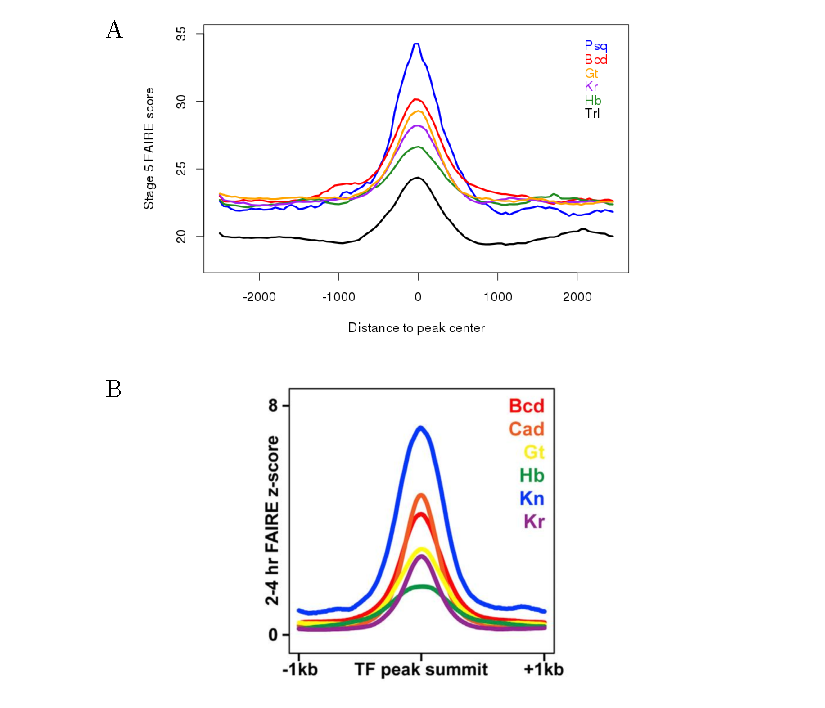
\includegraphics{fig6-8}
\caption{Enrichment of FAIRE read counts in TF binding peaks in \emph{D. pseudoobscura} and \emph{D. melanogaster}. A.) In \emph{D. pseudoobscura}, a 5-kb region around the center of each ChIP-seq peak for Psq, Bcd, Gt, Kr, Hb and Trl was considered, and the number of FAIRE-seq reads overlapping 50-bp bins in each interval was counted. FAIRE scores represent the average counts from Stage 5 replicate 3 in all peaks. A local maximum of FAIRE accessibility is seen at the center of the intervals for all TFs, with the highest scores varying between TFs. The highest FAIRE scores are found in Psq peaks, while the lowest are found in Trl peaks. B.) The order of the AP factors Bcd, Gt, Kr and Hb by FAIRE scores is the same as that found in \emph{D. melanogaster}. Figure reproduced from \citet{mckay_common_2013}.}
\label{Figure 6.8}
\end{figure}

\subsection{Relationship between FAIRE accessibility and Dichaete binding in \emph{D. pseudoobscura}}
I was also curious to investigate the relationship between chromatin accessibility and Dichaete binding as measured by the DamID experiment that I performed in \emph{D. pseudoobscura}. There is evidence to suggest that, in \emph{D. melanogaster}, Dichaete binds to HOT regions, which are associated with Trl binding and open chromatin \citep{aleksic_role_2013,kvon_hot_2012}. If Dichaete binding is partially driven by patterns of chromatin accessibility, then changes in accessibility between \emph{D. melanogaster} and \emph{D. pseudoobscura} may underscore some changes in binding between the two species, possibly leading to new functional binding events. In order to examine this relationship, I followed the same procedure as above, finding the center of each Dichaete-Dam binding interval and calculating the coverage of FAIRE-seq reads in 50-bp bins extending 2.5 kb on either side. This approach is not ideal for DamID, as the center of each binding interval does not necessarily correspond to the actual location of TF binding. However, by examining 5-kb intervals, the majority of true binding sites should be captured, as most GATC fragments are shorter than 5 kb. I calculated the average FAIRE scores in all intervals using all three biological replicates from each developmental stage separately, since the Dichaete-Dam experiment used embryos spanning all of the stages that were assayed using FAIRE-seq.\\

\begin{figure}
\centering
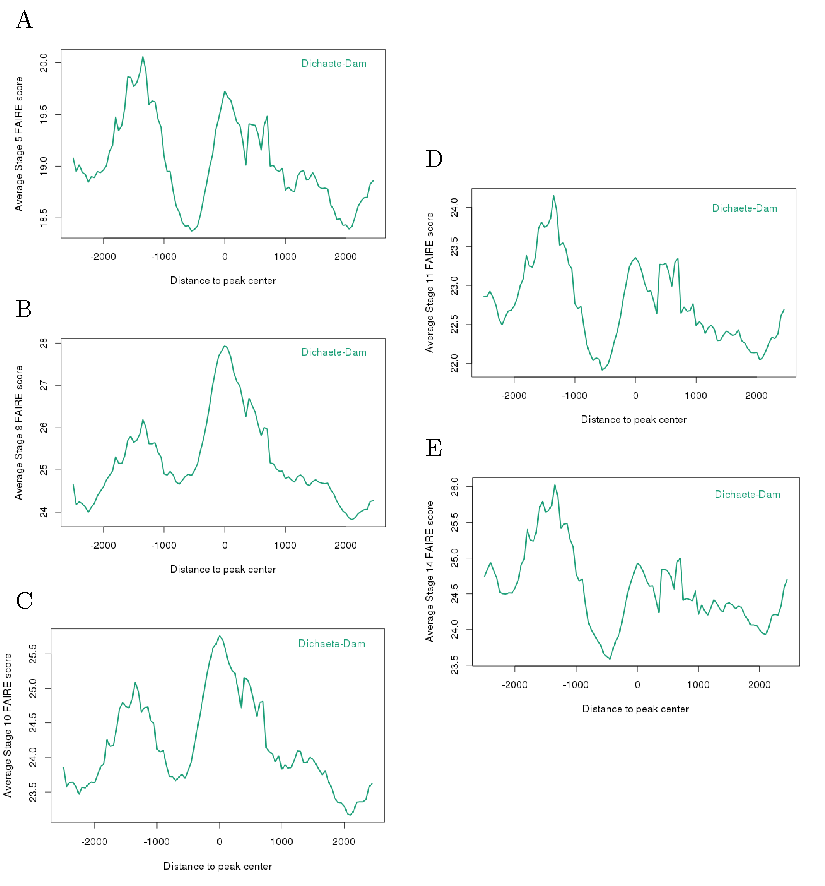
\includegraphics{fig6-9}
\caption{Enrichment of FAIRE read counts in Dichaete-Dam binding intervals in \emph{D. pseudoobscura}. A 5-kb region around the center of each binding interval was considered, and the number of FAIRE-seq reads overlapping 50-bp bins in each interval was counted. FAIRE scores represent the average counts from three replicates at each stage in all Dichaete-Dam intervals. In all stages, a peak of FAIRE accessibility is visible at about 1500 bp upstream of the center of the binding intervals, and another is visible at the center of the binding intervals. The peak at the center of the binding intervals is the strongest in stages 9 and 10. A.) Stage 5 FAIRE scores in Dichaete-Dam intervals. B.) Stage 9 FAIRE scores in Dichaete-Dam intervals. C.) Stage 10 FAIRE scores in Dichaete-Dam intervals. D.) Stage 11 FAIRE scores in Dichaete-Dam intervals. E.) Stage 14 FAIRE scores in Dichaete-Dam intervals.}
\label{Figure 6.9}
\end{figure}

The profiles of average FAIRE scores within Dichaete-Dam binding intervals are quite jagged and contain multiple peaks, which may be reflective of the fact that the strongest binding does not necessarily take place at the center of intervals. However, two main peaks of FAIRE accessibility are visible at each developmental stage, one located at around 1500 bp upstream of the interval centers and one coinciding with the center of the intervals (Figure 6.9). The relative heights of these peaks vary with developmental stage; the peak at the center of the intervals is the highest at stages 9 and 10 and decreases in stages 11 and 14. The absolute FAIRE scores around the center of binding intervals are also highest in stages 9 and 10, suggesting that Dichaete binding correlates best with chromatin accessibility during these stages. The overall shapes of the FAIRE profiles in Dichaete-Dam binding intervals are similar for all stages, which is not surprising given the high correlations between FAIRE accessibility profiles at all stages. The peaks of chromatin accessibility found in Dichaete-Dam intervals do not have as high FAIRE scores as for some other TFs, including Psq, Bcd and Gt; however, they are consistent with the FAIRE scores found in Trl and Hb peaks (Figure 6.8). In contrast to the pattern of FAIRE signal in Dichaete-Dam binding intervals, the intervals that are bound more highly by the Dam-only control in \emph{D. pseudoobscura} show lower FAIRE scores overall in each stage and do not show a peak of enrichment around the interval centers (Figure 6.10). These results suggest that, although FAIRE accessibility shows a complex pattern of enrichment within Dichaete-Dam binding intervals, functional Dichaete binding does correlate with chromatin accessibility to some extent in \emph{D. pseudoobscura}.\\

\begin{figure}
\centering
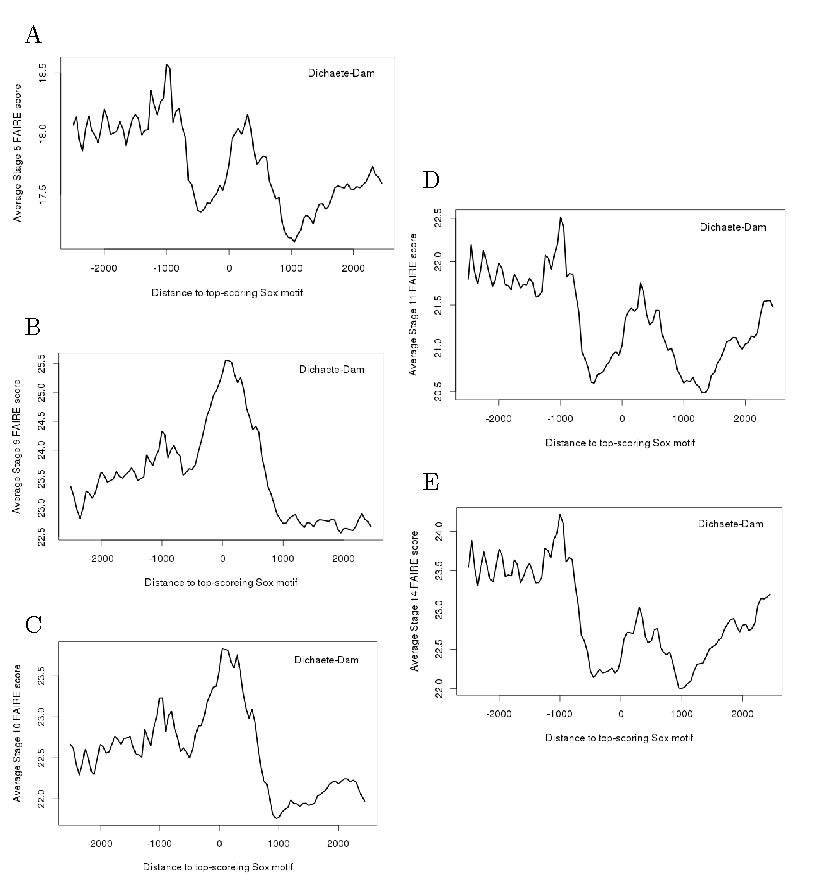
\includegraphics{fig6-10}
\caption{Enrichment of FAIRE read counts around Sox motifs in Dichaete-Dam binding intervals in \emph{D. pseudoobscura}. A 5-kb region centered around the best-scoring Sox motif in each binding interval was considered, and the number of FAIRE-seq reads overlapping 50-bp bins in each interval was counted. FAIRE scores represent the average counts from three replicates at each stage in all Dichaete-Dam intervals. In all stages, a peak of FAIRE accessibility is visible at about 1000 bp upstream of the Sox motifs, and another is visible centered around the Sox motifs. The peak centered around Sox motifs is the strongest in stages 9 and 10; however, in all stages it is weaker than the peak observed at the center of binding intervals. A.) Stage 5 FAIRE scores in Dichaete-Dam intervals. B.) Stage 9 FAIRE scores in Dichaete-Dam intervals. C.) Stage 10 FAIRE scores in Dichaete-Dam intervals. D.) Stage 11 FAIRE scores in Dichaete-Dam intervals. E.) Stage 14 FAIRE scores in Dichaete-Dam intervals.}
\label{Figure 6.10}
\end{figure}

Because DamID peaks do not necessarily contain true binding sites at their centers, I repeated the preceding analysis using peaks defined as 2.5kb up- and downstream from the coordinates of the highest-scoring match to a Sox motif in each interval. This definition of a peak is also somewhat problematic, as there were often more than one Sox motif with equally high or very close scores, and it is impossible to know from this dataset whether only one or more than one motif was bound in each binding interval. Again, the profiles of FAIRE accessibility scores in these peaks are quite jagged, although they do show a peak of enrichment near the center. This centered accessibility is most noticeable in stages 9 and 10; in both stage 5 and later stages, it appears to shift slightly downstream of the center, while another, more upstream peak of FAIRE accessibility is dominant (Figure 6.11). The FAIRE scores are lower overall in these motif-defined Dichaete-Dam peaks compared to the peaks defined around the centers of binding intervals, suggesting that, although there is some enrichment of accessibility at high-scoring Sox motifs, this approach does not capture the most accessible chromatin. Since the motif scores are based on a PWM constructed from the average of all motifs found, it is possible that the best-scoring motifs do not reflect actual motif usage by Dichaete, which may differ subtly in different populations of cells or different developmental stages. The variation in accessibility profiles observed in different stages might be a function of such differential motif usage.\\

\begin{figure}
\centering
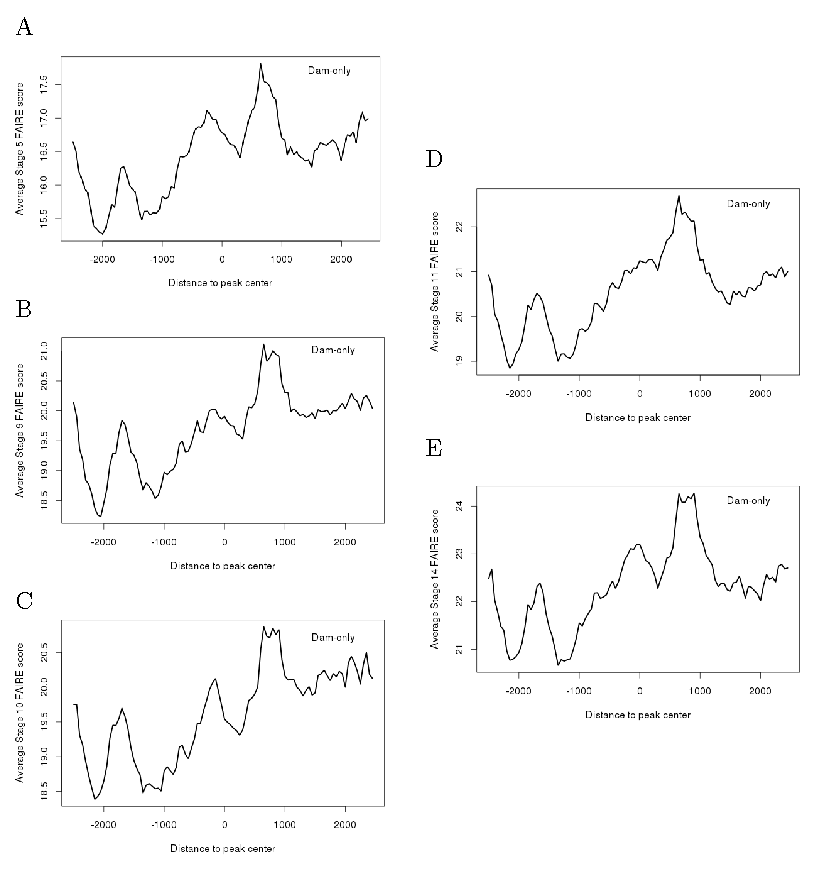
\includegraphics{fig6-11}
\caption{Average FAIRE scores in Dam-only binding intervals in \emph{D. pseudoobscura}. A 5-kb region around the center of each binding interval was considered, and the number of FAIRE-seq reads overlapping 50-bp bins in each interval was counted. FAIRE scores represent the average counts from three replicates at each stage in all Dichaete-Dam intervals. For each stage, the FAIRE scores in Dam-only control intervals are lower than the corresponding FAIRE scores in Dichaete-Dam intervals. Several local peaks of enrichment are present, but they are not located at the center of intervals. A.) Stage 5 FAIRE scores in Dam-only intervals. B.) Stage 9 FAIRE scores in Dam-only intervals. C.) Stage 10 FAIRE scores in Dam-only intervals. D.) Stage 11 FAIRE scores in Dam-only intervals. E.) Stage 14 FAIRE scores in Dam-only intervals.}
\label{Figure 6.11}
\end{figure}

I also used BedTools to find all intersections between Dichaete-Dam binding intervals and FDR10 FAIRE intervals in \emph{D. pseudoobscura} at each developmental stage. Although this approach is likely to underestimate the correlation between Dichaete-Dam binding and FAIRE accessibility, it allowed me to determine a set of Dichaete-Dam intervals that are definitively located in open chromatin. The numbers of Dichaete-Dam intervals that overlap with a FAIRE interval in each stage correspond to the average FAIRE scores in Dichaete-Dam intervals in each stage, with the highest numbers of overlaps present in stages 9 and 10 and the lowest numbers in stages 11 and 14 (Table 6.5). In total there are 257 unique Dichaete-Dam intervals detected that are located within a FAIRE interval, representing 8.7\% of all \emph{D. pseudoobscura} Dichaete-Dam binding intervals.\\ 

\begin{table}[h]
\centering
\begin{tabular}{|l|p{3cm}|p{3cm}|p{3cm}|}
\hline
\textbf{Developmental Stage} & \textbf{Overlaps between Dichaete-Dam and FAIRE intervals} & \textbf{Percent of FAIRE intervals overlapping} & \textbf{Percent of Dichaete-Dam intervals overlapping} \\ \hline
Stage 5             & 96                                                & 2.1\%                                  & 3.3\%                                         \\ \hline
Stage 9             & 196                                               & 3.8\%                                  & 6.6\%                                         \\ \hline
Stage 10            & 188                                               & 3.7\%                                  & 6.4\%                                         \\ \hline
Stage 11            & 48                                                & 1.1\%                                  & 1.6\%                                         \\ \hline
Stage 14            & 50                                                & 1.1\%                                  & 1.7\%                                         \\ \hline
\end{tabular}
\caption{Overlaps between Dichaete-Dam binding intervals and FAIRE intervals in \emph{D. pseudoobscura} embryos at five developmental stages.}
\label{Table 6.5}
\end{table}

In order to evaluate whether Dichaete-Dam binding intervals in FAIRE intervals tend to be unique to \emph{D. pseudoobscura} or conserved across species, I first found the set of binding intervals that are qualitatively conserved between \emph{D. melanogaster} and \emph{D. pseudoobscura}, as well as those that are unique to \emph{D. pseudoobscura}, and then translated their genomic coordinates to the \emph{D. pseudoobscura} genome assembly. This resulted in the loss of some intervals, as not all coordinates could be uniquely re-mapped; however, it was necessary in order to examine the effect of FAIRE accessibility in the \emph{D. pseudoobscura} genome. 1111 conserved intervals and 447 unique intervals were translated; 151 of the conserved intervals are located in a FAIRE interval, while only 12 of the unique \emph{D. pseudoobscura} intervals are located in a FAIRE interval (Figure 6.12). While the total proportion of Dichaete-Dam binding intervals located in FAIRE intervals is low, these binding intervals are significantly more likely to be conserved in \emph{D. melanogaster} than to be unique to \emph{D. pseudoobscura} (Chi-squared test with Yates’ continuity correction, \(\chi\)\textsuperscript{2} = 39.3, d.f. = 1, p-value = 3.6e-10). This suggests that, rather than the evolution of new binding events being driven by changes in chromatin accessibility, Dichaete-Dam binding sites in accessible chromatin tend to be conserved across species. In \emph{D. melanogaster} embryos, regions of open chromatin as measured by both DNase-seq and FAIRE-seq are bound by multiple regulatory factors and are associated with developmental regulatory genes \citep{mckay_common_2013,thomas_dynamic_2011}. Considering the functional importance of these regions, there is likely to be selective pressure to maintain open chromatin domains at key regulatory loci during evolution, despite the chromosomal rearrangements that have occurred between \emph{D. melanogaster} and \emph{D. pseudoobscura}.

\begin{figure}
\centering
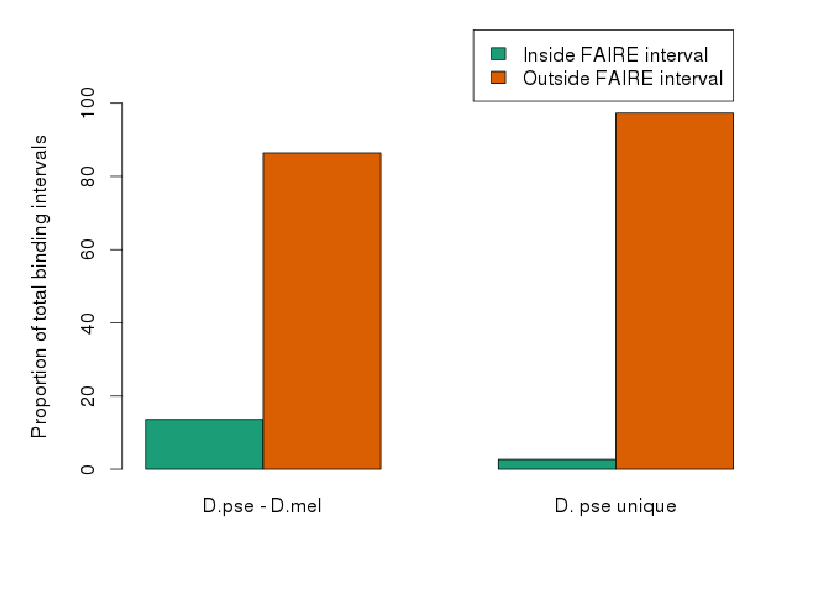
\includegraphics{fig6-12}
\caption{Dichaete-Dam binding intervals located within FAIRE intervals are more likely to be conserved than those located outside FAIRE intervals. Although the majority of Dichaete-Dam intervals do not overlap with a FAIRE interval in \emph{D. pseudoobscura}, those that do are significantly more likely to also be bound by Dichaete-Dam in \emph{D. melanogaster} compared to those that do not (p-value = 3.6e-10). Abbreviations: D. pse - D. mel, conserved in both \emph{D. pseudoobscura} and \emph{D. melanogaster}; D. pse unique, bound uniquely in \emph{D. pseudoobscura}.}
\label{Figure 6.12}
\end{figure}

\section{Comparison with chromatin accessiblity data in \emph{D. melanogaster}}
The two chromatin accessibility datasets in \emph{D. melanogaster} that offer the most direct comparison to my \emph{D. pseudoobscura} FAIRE-seq datasets are the DNase-seq data generated in five matching developmental stages by \citet{thomas_dynamic_2011} and the FAIRE-seq data generated by McKay \emph{et al.} \citep{mckay_common_2013} at 2-4 hours after egg laying, 6-8 hours after egg laying and 16-18 hours after egg laying. The McKay \emph{et al.} FAIRE-seq data are a better match in terms of technique, while the Thomas \emph{et al.} data are a more precise match in terms of temporal specificity; however, interesting comparisons can be made with both datasets. A simple comparison of the number of FAIRE and DHS peaks called reveals that I found significantly fewer peaks for every stage in \emph{D. pseudoobscura} than were found in \emph{D. melanogaster} for either technique. This is particularly the case for the DNase-seq dataset, in which 20,000-30,000 DHS peaks were called for each stage, or 5-6 times more than I found. McKay \emph{et al.} found 11,000-13,000 FAIRE peaks for each stage in \emph{D. melanogaster}, which are considerably fewer than the DHS peaks but still more than twice the number of FAIRE peaks called for \emph{D. pseudoobscura}. It is unclear why this is the case; it seems unlikely that the the \emph{D. pseudoobscura} genome genuinely has 2-6 times less open chromatin than the \emph{D. melanogaster} genome, as they have similar sizes and gene densities \citep{richards_comparative_2005}.\\ 

The FAIRE peaks in \emph{D. melanogaster} also overlap with a higher proportion of TF binding peaks than those identified in \emph{D. pseudoobscura} \citep{mckay_common_2013}; this may be due to an under-identification of FAIRE accessible regions in \emph{D. pseudoobscura} embryos, rather than a difference in the relationship between TFs and accessible chromatin between species. These differences could result in part from differences in the analytical methods used to process the data and call peaks; however, inspecting the read density profiles by eye suggests that the salient peaks have been successfully called for each dataset. Finally, the difference in numbers of peaks could be due to technical variation in the FAIRE protocol. It is possible that the \emph{D. pseudoobscura} embryos were underfixed, leading to a relative homogenization of signal and loss of peaks. On the other hand, if the embryos were overfixed, genuinely accessible regions might not have been recovered. Nonetheless, and encouragingly, despite the decreased numbers of peaks called in \emph{D. pseudoobscura}, the peaks that are called share similar properties to those identified in \emph{D. melanogaster} in terms of genomic annotations and TF binding patterns.\\

To measure the similarities between FAIRE-seq and DNase-seq datasets at each stage, I downloaded the Thomas \emph{et al.} DNase-seq data from the NCBI Sequence Read Archive [SRA:SRX020691, SRA:SRX020692, SRA:SRX020693, SRA:SRX020694, SRA:SRX020695, SRA:SRX020696, SRA:SRX020697, SRA:\\
SRX020698, SRA:SRX020699, SRA:SRX020700] and mapped the data against the \emph{D. melanogaster} genome. I then calculated the correlations between reads from each set of DNase-seq biological replicates and FAIRE-seq biological replicates that had been translated to the \emph{D. melanogaster} genome in the full set of DNase accessible regions, a total of 65536 intervals \citep{thomas_dynamic_2011}. For each stage, the DNase-seq replicates are highly correlated (R\textsuperscript{2} > 0.98), as are the FAIRE-seq replicates (R\textsuperscript{2} > 0.94). The correlations between FAIRE-seq replicates and DNase-seq replicates range from 0.55 to 0.71, with the highest correlations being present at stage 9. The differences between these samples encompass both technical differences between FAIRE-seq and DNase-seq as well as differences in patterns of accessibility between species; however, the coefficients of correlation are similar to those calculated for Dichaete-Dam binding between \emph{D. melanogaster} and \emph{D. pseudoobscura}, showing that a similar amount of inter-species variation is captured by examining chromatin accessibility as by examining the binding patterns of a single TF. Clustering all replicates from both techniques at all stages shows that FAIRE-seq samples are more similar across stages than DNase-seq samples (Figure 6.13). For some stages, such as stage 14, there are higher correlations between samples from the two techniques than there are between samples from different stages; however, overall, the high degree of similarity between FAIRE-seq stages means that the FAIRE-seq samples show similar correlations to DNase-seq samples at all stages.\\

\begin{figure}
\centering
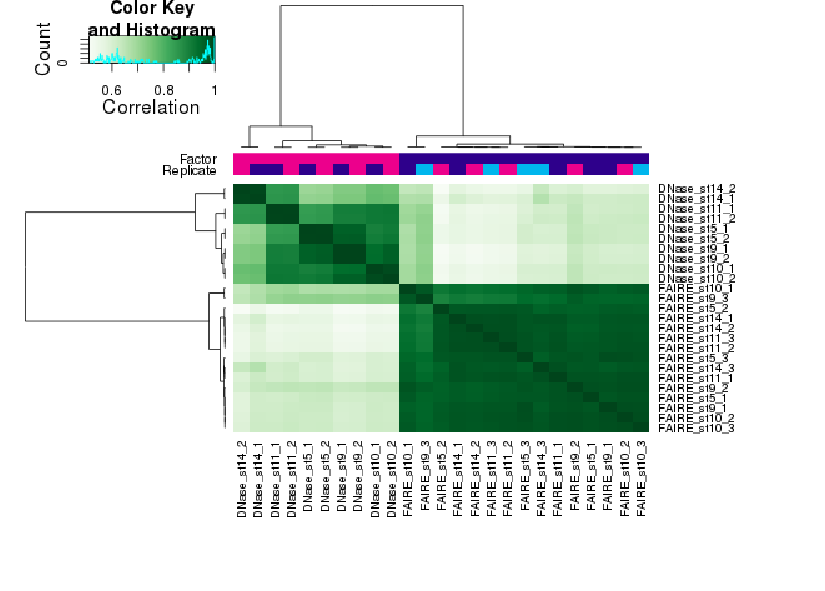
\includegraphics{fig6-13}
\caption{Heatmap showing correlations between translated FAIRE-seq sample read counts and DNase-seq sample read counts within all DNase accessible sites in five developmental stages in \emph{D. melanogaster}. FAIRE-seq samples show higher correlations between stages than DNase-seq samples. The highest correlations between techniques are for FAIRE-seq samples from stages 9 and 10 with all DNase-seq samples. The color key and histogram show the distribution of pairwise correlations between sample affinity scores in all DNase accessible regions. Darker green corresponds to a higher correlation, while lighter green corresponds to a lower correlation.}
\label{Figure 6.13}
\end{figure}

I performed the same type of analysis with the McKay \emph{et al.} FAIRE-seq samples from \emph{D. melanogaster} embryos, which I also downloaded from the NCBI Sequence Read Archive [SRA:SRX155022, SRA:SRX155023, SRA:SRX155024] and mapped against the \emph{D. melanogaster} genome. I calculated the correlations between reads from each McKay et al. FAIRE-seq sample and each of my translated FAIRE-seq samples from overlapping stages (stage 5 versus 2-4 hour embryos, stage 9, 10 and 11 versus 6-8 hour embryos and stage 14 versus 16-18 hour embryos) within the McKay FAIRE accessible regions. In each comparison, the \emph{D. pseudoobscura} FAIRE-seq replicates show considerably higher correlations, ranging from 0.92 - 0.97, than the McKay FAIRE-seq replicates, whose correlations ranged from 0.58 - 0.77. The one outlier for the \emph{D. pseudoobscura} FAIRE-seq samples was stage 5 replicate 1, which showed poor correlations with the other stage 5 replicates in the regions examined. With the exception of that sample, the \emph{D. pseudoobscura} FAIRE-seq samples show similar but slightly lower levels of correlation with the McKay FAIRE-seq samples compared to the DNase-seq samples, ranging from 0.43 - 0.60 for 2-4 hour embryos (Figure 6.14A), 0.48 - 0.60 for 6-8 hour embryos (Figure 6.14B) and 0.36 - 0.56 (Figure 6.14C). For the latest stage embryos, replicate 1 correlates more closely with the \emph{D. pseudoobscura} stage 14 samples than does replicate 2. While it is somewhat surprising that the samples from two FAIRE-seq experiments are less correlated than samples from a FAIRE-seq experiment and a DNase-seq experiment, even between different stages, this may be due to the fact that fewer peaks were identified in the McKay FAIRE-seq data and so less of the data was included in calculating the coefficients of correlation, which may have resulted in the exclusion of some relevant genomic regions.

\begin{figure}[H]
\centering
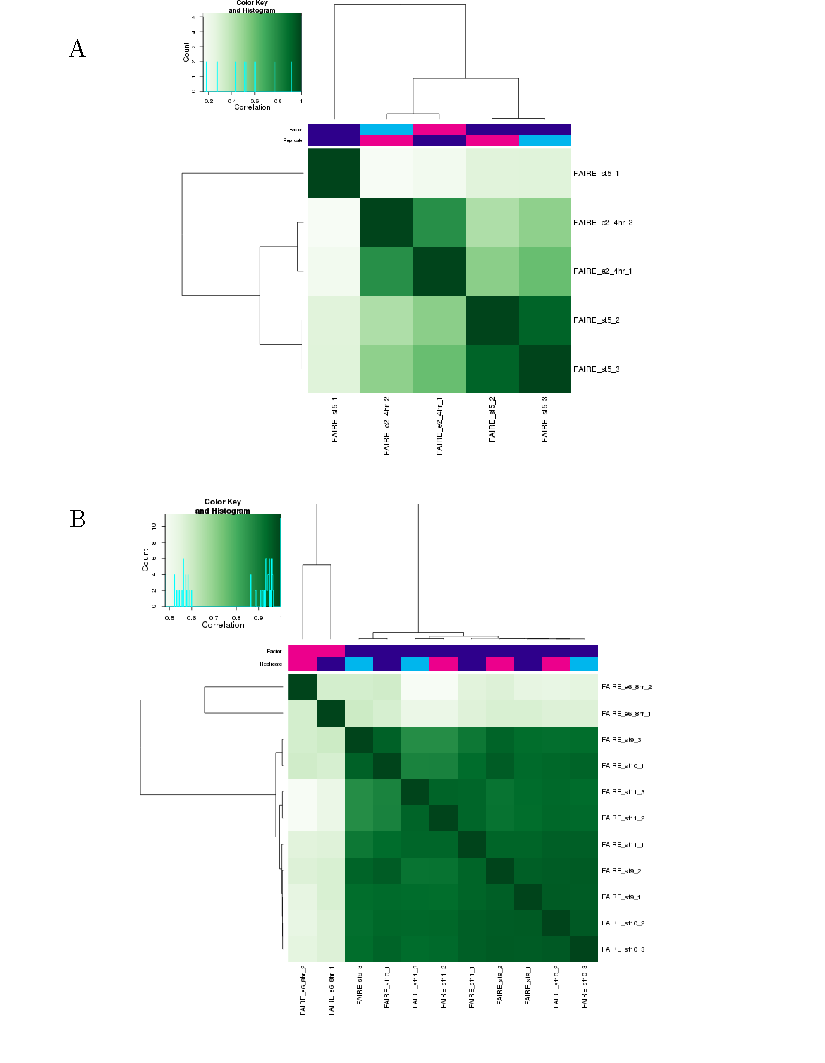
\includegraphics{fig6-14a}
\label{Figure 6.14}
\end{figure}

\begin{figure}[H]
\centering
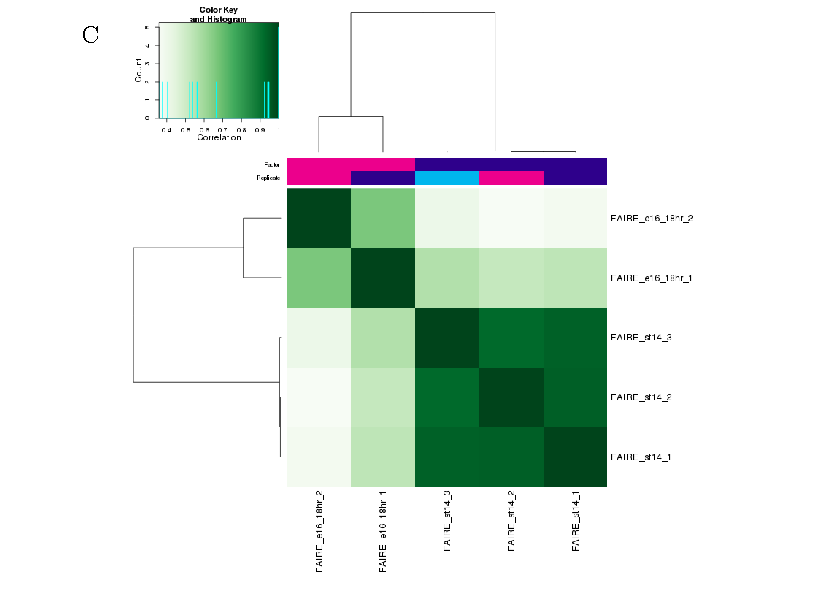
\includegraphics{fig6-14c}
\caption{Heatmaps showing correlations between translated \emph{D. pseudoobscura} FAIRE-seq sample read counts and \emph{D. melanogaster} FAIRE-seq sample read counts from McKay \emph{et al}. (2013) within all \emph{D. melanogaster} embryonic FAIRE accessible sites. The color key and histogram show the distribution of pairwise correlations between sample affinity scores in all FAIRE accessible regions. Darker green corresponds to a higher correlation, while lighter green corresponds to a lower correlation. A.) Comparison of stage 5 translated FAIRE-seq samples from \emph{D. pseudoobscura} and 2-4 hour FAIRE-seq samples from \emph{D. melanogaster}. \emph{D. pseudoobscura} stage 5 replicate 1 is a clear outlier. B.) Comparison of stage 9, stage 10 and stage 11 translated FAIRE-seq samples from \emph{D. pseudoobscura} and 6-8 hour FAIRE-seq samples from \emph{D. melanogaster}. The \emph{D. pseudoobscura} samples show higher correlations, even across stages, than do the \emph{D. melanogaster} replicates. C.) Comparison of stage 14 translated FAIRE-seq samples from \emph{D. pseudoobscura} and 16-18 hour FAIRE-seq samples from \emph{D. melanogaster}. \emph{D. melanogaster} replicate 1 is more similar to all of the \emph{D. pseudoobscura} samples than is replicate 2.}
\label{Figure 6.14}
\end{figure}

\section{Discussion of results}
The FAIRE-seq datasets which I generated for five developmental stages in \emph{D. pseudoobscura} embryos show very high levels of reproducibility between replicates, as well as high correlations between developmental stages. The majority of accessible sites identified originate in stage 5 and are maintained throughout development, although some developmentally dynamic sites originate and are lost in later stages. These samples show significant differences from publicly available chromatin accessibility datasets in \emph{D. melanogaster}, some of which seem more likely to be due to technical differences in sample preparation than to biological differences. My \emph{D. pseudoobscura} FAIRE-seq data contains 2-6 times fewer highly accessible regions in each developmental stage, and these regions contain fewer overlaps with TF binding intervals in \emph{D. pseudoobscura}, measured either through ChIP-seq or DamID. Additionally, there are fewer peaks of accessibility identified as unique to each stage in \emph{D. pseudoobscura} than in \emph{D. melanogaster}; however, again, this may be due to technical differences resulting in a loss of more developmentally dynamic accessible regions. On the level of read counts, however, the \emph{D. pseudoobscura} samples show similar levels of correlation with \emph{D. melanogaster} DNase-seq samples as do \emph{D. pseudoobscura} Dichaete-Dam samples with \emph{D. melanogaster} Dichaete-Dam samples. They show slightly lower levels of correlation with \emph{D. melanogaster} FAIRE-seq samples, which, although they were detected using the same technique, span different periods of developmental time. The read-level correlations suggest that, while a comparison of thresholded peaks may highlight technical differences, the overall accessibility profiles of \emph{D. pseudoobscura} embryonic chromatin and \emph{D. melanogaster} embryonic chromatin have evolved differences at a similar rate as the binding profiles of several transcription factors, as well as the insulator protein CTCF, between these two species \citep{he_high_2011,ni_adaptive_2012,paris_extensive_2013}.\\

In terms of annotation to genomic features and TF binding, the \emph{D. pseudoobscura} FAIRE intervals show similar overall properties to the \emph{D. melanogaster} FAIRE and DNase intervals. Although the quality and level of detail of gene model predictions available for \emph{D. pseudoobscura} is lower than that for \emph{D. \\
melanogaster}, a similar proportion of the \emph{D. pseudoobscura} FAIRE intervals and the \emph{D. melanogaster} DNase intervals are annotated to intergenic DNA and, for the GeneID gene predictions, intronic DNA. The gene border category in \emph{D. pseudoobscura} may include TSSs as well as 5’ UTRs and 3’ UTRs; the DNase intervals are annotated to these categories at a combined proportion that is close to that of \emph{D. pseudoobscura} FAIRE intervals in gene borders. The biggest difference between the genomic annotations in the two species is that a higher proportion of \emph{D. melanogaster} DNase intervals are annotated to coding sequences; however, these may include intervals that partially overlap exons as well as introns, which were annotated to the exon border category in \emph{D. pseudoobscura} \citep{thomas_dynamic_2011}.\\

Previous studies have indicated that DNase-seq tends to identify more open chromatin regions in promoters than FAIRE-seq \citep{koohy_chromatin_2013}. However, both the \emph{D. pseudoobscura} FAIRE intervals and the \emph{D. melanogaster} DNase intervals show a strong presence of promoter motifs, although different promoter motifs are enriched in each dataset \citep{thomas_dynamic_2011}. Many of the top known and \emph{de novo} motifs found in the \emph{D. pseudoobscura} FAIRE intervals were difficult to assign to a \emph{Drosophila} TF. However, there is a strong enrichment for motifs corresponding to several major families of DNA binding domains, including the NHR, HLH, bZIP and zf families. This indicates that, in addition to promoters, FAIRE accessible regions include enhancers that are bound by a broad variety of regulatory factors. In support of this view, a peak of FAIRE signal was found in the center of ChIP-seq binding intervals for several AP factors in \emph{D. pseudoobscura}, including Bcd, Gt, Kr and Hb, as well as the TFs Psq and Trl, which are both implicated in chromatin remodelling. Interestingly, the relative intensities of FAIRE signal in AP factor binding intervals follow the same order in \emph{D. pseudoobscura} embryos as in \emph{D. melanogaster} embryos \citep{mckay_common_2013}.\\

One of the main motivations behind generating a FAIRE-seq dataset in \emph{D. pseudoobscura} was to investigate the relationship between accessible chromatin and conservation of group B Sox binding, using the DamID data that I acquired in \emph{D. pseudoobscura} and \emph{D. melanogaster}. Since I was not able to perform DamID for SoxNeuro in \emph{D. pseudoobscura}, I focused this analysis on Dichaete-Dam binding. First, I examined the overall pattern of FAIRE accessibility in Dichaete-Dam binding intervals in \emph{D. pseudoobscura}. I found that, although the FAIRE scores in Dichaete-Dam intervals are not as high as for some other TFs, there is an enrichment of FAIRE accessibility both in the center of Dichaete-Dam intervals and approximately 1.5 kb upstream of the center. The average profiles of FAIRE scores in Dichaete-Dam intervals are complex, reflecting the fact that DamID binding intervals are not necessarily centered around the true binding site, and vary with developmental stage; the highest peak of FAIRE signal in the center of Dichaete-Dam intervals is present at stage 9. The intervals that are more highly bound by the Dam-only control also have a complex FAIRE signal profile; however, they do not show a peak of accessibility at their center, and their FAIRE scores are lower on average than those in Dichaete-Dam intervals, suggesting that accessibility is more strongly related to functional TF binding. I also found the overlaps between Dichaete-Dam binding intervals and FDR10 FAIRE intervals in each stage. Although only a small percentage of intervals are directly overlapping, the numbers of overlaps in each stage correspond to the FAIRE signal profiles, with the highest number overlaps also present at stage 9. These results suggest that, although Dichaete-Dam binding may not take place in the accessible regions that are most strongly identified by FAIRE-seq, there is a correlation between chromatin accessibility and Dichaete binding.\\

In the case of the Dichaete-Dam intervals that do overlap with FAIRE accessible regions in \emph{D. pseudoobscura}, I wondered if these intervals were more likely to be uniquely bound in \emph{D. pseudoobscura} or if binding was conserved at orthologous sites in \emph{D. melanogaster}. Since the \emph{D. pseudoobscura} genome has undergone substantial rearrangements since its split from a common ancestor with \emph{D. melanogaster}, it seemed feasible that newly-evolved accessible regions in the \emph{D. pseudoobscura} genome might underpin the evolution of lineage-specific TF binding events. However, I found that very few \emph{D. pseudoobscura} Dichaete-Dam binding intervals located in FAIRE intervals are unique to \emph{D. pseudoobscura}. On the contrary, they are significantly more likely to be conserved in \emph{D. melanogaster}, while Dichaete-Dam binding intervals that are not located in FAIRE intervals are more likely to be uniquely bound (Figure 6.12). While it is still possible that the uniquely bound Dichaete-Dam intervals within FAIRE accessible regions evolved in tandem with rearrangements of chromatin domains, it appears that selective pressure on functional enhancers may act to maintain both open chromatin and Dichaete binding sites between species of \emph{Drosophila}.\\

In this chapter and the preceding ones, I have presented the major datasets that I generated during my Ph.D., which consist of DamID binding datasets for Dichaete in four species of \emph{Drosophila} and SoxNeuro in two species of \emph{Drosophila} as well as FAIRE-seq datasets for five developmental stages in \emph{D. pseudoobscura}. Transcription factor binding and chromatin accessibility have been shown to be highly correlated in \emph{D. melanogaster}, with chromatin accessibility highlighted as a potential driver of TF binding patterns \citep{kaplan_quantitative_2011, li_role_2011}. While several comparative studies of TF binding have been performed in various \emph{Drosophila} species, chromatin accessibility in non-model species has not previously been examined. Although my FAIRE-seq samples may have suffered from some technical problems resulting in the identification of significantly fewer peaks than for similar experiments in \emph{D. melanogaster}, the biological replicates show extremely high reproducibility, suggesting that the peaks that were identified represent true open chromatin. Combining a comparative study of TF binding and chromatin accessibility allowed me to discover the fact that \emph{D. pseudobscura} Dichaete-Dam binding intervals located in open chromatin are significantly more likely to be conserved in \emph{D. melanogaster} compared to those that are not located in open chromatin, which supports the functional relationship between chromatin accessibility and TF binding. In the following chapter, I will discuss the conclusions that can be drawn from all of these datasets in the context of the ongoing debate over what constitutes functional regulatory DNA, as well as presenting my vision for future directions.

